%%This is the KMD un-official thesis template (Engineering Format for English Writer).
%
\documentclass[12pt,a4paper]{report}  % Should work with either pLaTeX or XeLaTeX
\usepackage{style/new-emthesis}
%
%%%%%%%%%%%%%%%%%%%%%%%%%%%%
%
% Decide what graphicx driver to use for images.
% For pLaTeX should use 'dvipdfmx'; default is OK otherwise.
\newcommand\gfxdriver{}
\ifXeTeX                        %% If XeLaTeX is being used
    \usepackage{fontspec}
    % Use standard TeX ligature logic
    \defaultfontfeatures{Ligatures=TeX}
    % Enable use of XeTeX CJK fonts for Japanese text if needed
    \usepackage[indentfirst=false]{xeCJK}
    % XeLaTeX also requires specifying CJK fonts
    %   (these must be TTF/OTF fonts installed on the computer)
    \setCJKmainfont{IPAMincho}      % Japanese serif (Mincho) font - e.g. MS PMincho
    \setCJKsansfont{IPAPGothic}     % Japanese sans (Gothic) font - e.g. MS PGothic
    \setCJKmonofont{IPAGothic}      % Japanese monospaced font - e.g. MS Gothic

\else\ifptex                    %% If pLaTeX is being used
    % Uncomment next 2 lines to enable ruby characters (furigana) if needed
    %\usepackage{pxrubrica}
    %\rubysetup{g}

    \renewcommand\gfxdriver{dvipdfmx}
\fi\fi
\usepackage[\gfxdriver]{graphicx}
%
%%%%%%%% Load other packages
\usepackage{mathrsfs}
\usepackage{amsmath}
\usepackage{listings}
\usepackage{color}
\usepackage{siunitx}
\usepackage{subfigure}
\usepackage{tabularx}
\usepackage{longtable}
\usepackage{multirow}
\usepackage{fancybox}
\usepackage{amssymb}
\usepackage{moreverb}
\usepackage{afterpage}
\usepackage{cite}
%\usepackage{harvard-oikos}
\usepackage{style/ccaption}           % caption
\usepackage{style/fn2end}             % footnotes script
\usepackage{style/fn2end_config}      % footnotes edit script
\usepackage{tabu}               % more powerful/flexible tables
\usepackage{fancyhdr}           % used to enable nice page headers
\ifptex
    \usepackage[hyphens]{url}           % format URLs nicely
\else                                   % also create links in document
    \usepackage[hidelinks,hypertexnames=false,hyperfootnotes=false]{hyperref}
    % Uncomment to enable ruby characters (furigana) if needed
    %\ifXeTeX \usepackage[CJK,nooverlap]{ruby} \fi
\fi

\lstset{frame=tb,
  aboveskip=3mm,
  belowskip=3mm,
  showstringspaces=false,
  columns=flexible,
  basicstyle={\small\ttfamily},
  numbers=none,
  numberstyle=\tiny\color{gray},
  keywordstyle=\color{blue},
  commentstyle=\color{dkgreen},
  stringstyle=\color{mauve},
  breaklines=true,
  breakatwhitespace=true,
  tabsize=3
}

%
%%%%%%%%%% Other tweaks
\makeatletter
%
% Remove the number from subsection headings
%\renewcommand*{\l@subsection}{\@dottedtocline{2}{3.8em}{1.2em}}
%\renewcommand{\thesubsection}{\hskip-1.0em}
%
% Make in-page footnotes use regular numbers instead of superscripts (per CMS)
\renewcommand{\@makefntext}[1]{%
    \noindent
	\leftskip=1.5em
	\hskip-1.5em
	\makebox[1.5em][l]{\@thefnmark}{#1}
}
\setlength{\skip\footins}{\baselineskip}
\setlength{\footnotesep}{1.3em}
%
% Also use a tighter line spacing for endnotes
\let\saved@theendnotes\theendnotes
\renewcommand{\theendnotes}{%
    \setlength{\baselineskip}{1.3em}
	\saved@theendnotes
}
%
% Uncomment the following to include the abstract in the table of contents:
%\let\saved@eabstractpage\eabstractpage
%\renewcommand{\eabstractpage}{%
%    \addcontentsline{toc}{chapter}{\abstractname}
%    \saved@eabstractpage
%}
\makeatother
%%%%%%%%%%%%%%%%%%%%%%%%%%%%

%
%%%%%%%%%%
% Page Style Settings - Choose One
\pagestyle{final}               % Final Draft
%\pagestyle{draft}               % Drafts


%%%%%%%%%%%%%%%%%%%%%% Optional Styling Tweaks %%%%%%%%%%%%%%%%%%%%%%
%
% Uncomment one of these to change the default Latin font:
%\renewcommand*\rmdefault{bch}   % Charter
%\renewcommand*\rmdefault{pnc}   % Century Schoolbook

%
% Uncomment to adjust the default line spacing.  The defaults are 1.1 for
% English and 1.2 for Japanese.  For tighter spacing, 1.0 can be used.
%\renewcommand{\baselinestretch}{1.0}

%
% Add a nice header to each non-initial page (optional):
%
\pagestyle{fancy}
\setlength{\headheight}{13.6pt}
\renewcommand{\chaptermark}[1]{\markboth{\MakeUppercase{#1}}{}}
\renewcommand{\sectionmark}[1]{\markright{\thesection\hspace{1em}#1}}
\fancyhead{}
\makeatletter\if@twoside              % Two-sided (book) style layout
    \fancyhead[LE]{\footnotesize\leftmark}   % Chapter name on left-hand page
    \fancyhead[RO]{\footnotesize\rightmark}  % Section name on right-hand page
\else                                 % Regular (single-page) layout
    \fancyhead[L]{\footnotesize\leftmark}    % Chapter name at left side
    \fancyhead[R]{\footnotesize\rightmark}   % Section name at right side
\fi\makeatother

%
% Table padding for use with tabu (only if \usepackage{tabu} specified above)
\setlength{\tabulinesep}{3pt}   % Vertical padding between rows

%
% Adjust space around float captions
\setlength{\abovecaptionskip}{0.5em}    % Space above bottom captions
\setlength{\belowcaptionskip}{1em}      % Space below top captions

%
%%%%%%%%%%%%%% Thesis Parameters - Edit as Appropriate %%%%%%%%%%%%%%
%
%
% Language Settings
%\lang{Japanese} % Japanese
\lang{English} % English

%
% Student ID number
\studentnumber{81923362}

%
% Choosing Masters Thesis or Report
\doctitle{\mastersthesis}       % Masters Thesis
%\doctitle{\mastersreport}      % Report
\graduateschool{Graduate School of Science and Technology}
\school{School of Integrated Design Engineering}
%
% What Degree to obtain
\major{\mediadesign}    % Degree of Media Design

% \graduateschool{}
%
% Title (in LaTeX)
\etitle{Numerical investigation on electrical and thermal characteristics in organic semiconductor films from the aspect of variable range hopping}
%
% Title (in plain text)
%   No need to set if the same as  (in LaTeX)
\eptitle{}

%
%Author's Name (in LaTeX)
\eauthor{Descouens Nicolas}
%
% Author's Name (in plain text)
%   No need to set if the same as in (in LaTeX)
\epauthor{}
\advisor{Associate Professor Noda Kei}
%
% Academic Year
\syear{2021}
%\heiseiyear{24}            % only required for Japanese thesis
%\smonth{2}
%\sday{7}

%
% Advisors
%
%\echmembers{Professor Hideki Sunahara}{(Supervisor)}
%          {Professor Akira Kato}{(Co-supervisor)}
%
% Thesis committee members - Supervisor, Co-supervisor, and Member must be
% specified.  Uncomment and edit ONE of these depending on the total number:
%
% If 5 advisors:
% Supervisor, Co-supervisor, and Member must be specified.
%\ecomembers{Professor Shunsuke Uemura}{(Supervisor)}
%          {Professor Minoru Ito}{(Co-supervisor)}
%          {Associate Professor Masatoshi Yoshikawa}{(Member, Nagoya University)}
%          {Associate Professor xxxxxx xxxxxx}{(Member)}
%\eaddcomembers{Associate Professor oooooo oooooo}{(Member)}
%
% If 4 advisors:
%\ecomembers{Professor Hideki Sunahara}{(Supervisor)}
%          {Professor Akira Kato}{(Co-supervisor)}
%          {Professor Nobuo Kawaguchi}{(Member, Nagoya University)}
%          {Associate Professor xxxxxx xxxxxx}{(Member)}
%
% If 3 advisors:
% \advisor{Hideki Sunahara}
% If 2 advisors:
% \ecomembers{Professor Hideki Sunahara}{(Supervisor)}
%           {Professor Akira Kato}{(Co-supervisor)}
%
% 5 or 6 Keywords (in LaTeX)
%
\ekeywords{}
%
% 5 or 6 Keywords (in plain text)
%   No need to set if the same as in (in LaTeX)
%\epkeywords{Design Thinking, Creative Society, Workshop, Innovation, Education}

%
%Choose one submission category from [Design, Science / Engineering, Social Science / Humanities, Action Research]
\ecategory{Science / Engineering}
%Choose one submission category from [Design, Science / Engineering, Social Science / Humanities, Action Research] (in plain text)
\pecategory{Science / Engineering}


%%%%%%%%%%%%%%%%%%%%%%%%%%Abstract%%%%%%%%%%%%%%%%%%%%%%%%%%%%%%%%%
\eabstract{
}
%%%%%%%%%%%%%%%%%%%%%%%%% document starts here %%%%%%%%%%%%%%%%%%%%%%%%%%%%

%%%% No need to edit these

\begin{document}
%
%
\titlepage
\comemberspage
\firstabstract
%\secondabstract            % only required for Japanese thesis


%
%%%%%%%%%%%%%%%%%%%%%%%% Acknowledgements here %%%%%%%%%%%%%%%%%%%%%%%
\acknowledgements


%
%%%%%%%%%%%%%%%%%%%%%%%%%%%% Main Matter %%%%%%%%%%%%%%%%%%%%%%%%%%%%%
%
%Table of Contents and related matter
\toc
\newpage
\listoffigures
%
\newpage
\pagenumbering{arabic}

%
%%%%%%%% Chapters - input individual chapters here
%
% !TeX root = document-en.tex

\chapter{Introduction}
\label{chap:intro}

\makeendnotes  %make notes at the last of this chapter // if you do not  want use endnotes style, please comment out this.

\section{Organic semiconductors}

\subsection{Background}

For the past century, inorganic materials have been at the heart of the semiconductor industry, with element such as silicon, germanium or gallium arsenide. But, the industry turned itself to new devices and organics semiconductor are one of them. Their different set of properties: very flexible, low cost, less polluting helped them to gain interest.

More specifically, in 1977, the first highly conducting polymer was found, chemically doped polyacetylene, was discovered \cite{polyacetylene}. Such materials can be easily processed by techniques already know in the industry: vacuum evaporation, solution casting\dots But a better understanding and control of the self-assembly of molecules, as well as a booming research field, have increased greatly the performances, reaching the charge carrier mobility of amorphous silicon for some of them (fig. \ref{fig:1}). The high diversity of geometry within the material allows a better tuning of the characteristic of the semiconductor to the use. One greater advance is the combination of both organic and inorganic molecules, particularly with perovskite. The high mobility of inorganic material combined with the more flexible geometry of organic ones make possible the creation of devices that reaches the performances of single-crystal silicon \cite{IBM,perovskite}.

\begin{figure}
    \centering
    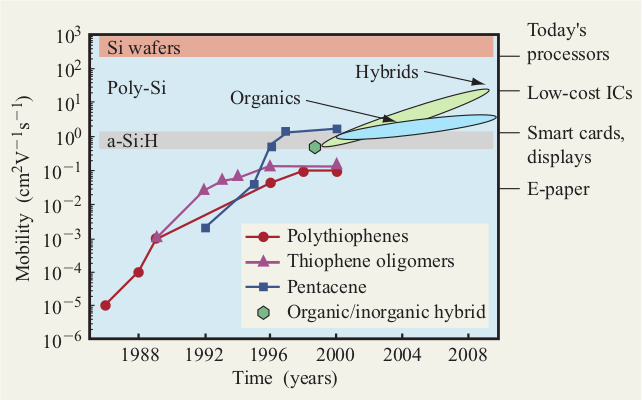
\includegraphics[width=.6\paperwidth]{figures/evolution_perf.png}
    \caption{Evolution of the performance for some organic semiconductors \label{fig:1}\cite{IBM}}
\end{figure}

This new development has been seen through the recent appearance of organic devices in the market. The more flagrant one is OLED devices, they offer a better diversity (flexible screens) with increased performance (higher color fidelity, darker black and better contrast) as well as consumption. But it's also used in professional devices such as OTFT \cite{OTFT}, laser diode \cite{laserDiode}, \dots

\subsection{Organic materials}

Organic molecule are bound to each other by $\pi - \pi$ bounding which are the result of $p_z$-orbitals of $sp^2$-hybridized C-atoms in the molecules (fig. \ref{fig:2}). Such bonding is way weaker compared to the classic $\sigma$-bounding in the molecule backbone. Therefore, the $\pi-\pi^*$ transitions have a typical lower gap: around $\SI{1.5}{eV}-\SI{3}{eV}$ (fig. \ref{fig:3}). Their crystallinity ranges from single-crystal (pentacene, rubrene crystals) \cite{mono_crystal} to completely amorphous semiconductors like $\alpha$-NPD \cite{amorphous}.

\begin{figure}
    \centering
    \includegraphics*[width=0.4\paperwidth]{figures/pi_bonding.png}
    \caption{$\sigma$ and $\pi$ bonds in ethene \label{fig:2} \cite{intro_orga}}
\end{figure}

\begin{figure}
    \centering
    \includegraphics*[width=0.4\paperwidth]{figures/pi_pistar.png}
    \caption{$\pi-\pi^*$ bonding \label{fig:3} \cite{intro_orga}}
\end{figure}

Those weaker Van der Waals bonding lead to more localized charge carrier in the material. Most of the time, charge carriers do not evolve in bands like in Si, but are subject to a HOMO (Highest Occupied Molecular Orbital) and LUMO (Lowest Unoccupied Molecular Orbital) states. It results in a much weaker wavefunction delocalization for the neighboring molecules \cite{intro_orga}. Instead of band transport, organic materials are subject to hopping transport: a charge carrier hop from a site to an other and thus participate to the general conduction (fig.\ref{fig:4}). The difference between trapping and hopping state is in the recombination and release rate. if the former one is higher than the letter one, the state is a recombination center, otherwise, it is a trap. In this model the difference between trapping states and recombination states can be thin.

\begin{figure}
    \centering
    \includegraphics*[width=0.4\paperwidth]{figures/hopping_theory.png}
    \caption{Hopping transport \label{fig:4}}
\end{figure}

Organic semiconductors are divided between polymers and small molecules. The separation occurs at $1000$ molecular weights. Small molecules can achieve high cristallinty but are less soluble in solvent, requiring dry processes such as vacuum deposit, which is more difficult and more costly. On the other hand, polymer are easier to made in organic solvents. Even though small molecules show better performances, they're less stable than polymer in atmospheric conditions.

\subsection{Charge carrier transport}

As it has been said before, disorganized organic semiconductors are the place of localized charge carrier transport, and in the 70's, a theory has been proposed involving tunneling between near states \cite{hopping_theory_1}. Such theory as been previously discovered by Mott based on the dependence of the mobility on the temperature: an increasing temperature leads to an increasing mobility. This relation has been verified in practical devices \cite{hopping_theory_1,multiple_theory}.

In the variable range hopping theory (VRH), the displacement between two states for a charge carrier is determined only by the difference in energy $W$ and in position $R$, thus highlighting the fact that our system is resolutely in 4D. On top of that, we assume that the system is so disordered that this two quantities are decoupled. The jump frequency is usually described by the Miller-Abrahams formalism \cite{miller}:

\begin{equation}
    \nu=\nu_{0}\left\{\begin{array}{r}
    \exp \left(-2 \alpha R_{i j}-\frac{E_{j}-E_{i}}{k_{B} T}\right): E_{j}-E_{i} \geq 0 \\
    \exp \left(-2 \alpha R_{i j}\right): E_{j}-E_{i} \leq 0
    \end{array}\right.
    \label{eq:1}
\end{equation}

\begin{itemize}
    \setlength\itemsep{0.1em}
    \item $\nu_0$: base-jump frequency
    \item $R_{i j}$: distance between initial state $i$ and final state $j$
    \item $\alpha$: decay constant of the assumed hydrogen-like localized state wave functions
    \item $E_i$: energy of the state $i$
\end{itemize}

Depending on the position of the final state $j$, the formula change. If the state is on higher energy, it requires tunneling to occur on the energetic part, whereas if the reaching state if of a lower energy, only the distance is taken into account for the tunneling effect.

Using this formalism, it is possible to access the mobility and diffusivity for charge carrier.

\subsection{The einstein relation}

\subsubsection{Classical einstein relation}

\begin{equation}
    \frac{D}{\mu} = \frac{k_bT}{q}
    \label{eq:2}
\end{equation}

\begin{itemize}
    \setlength\itemsep{0.0em}
    \item $\mu$: mobility
    \item $D$: diffusion
    \item $k_B$: Boltzmann constant
    \item $T$: temperature
    \item $q$: elementary charge
\end{itemize}

The einstein relation \cite{einstein}, is a useful equation that link two quantities, $\mu$ and $D$ over a simple equation. $D$ constitutes a key parameter in analyzing semiconductor but is not so easy to measure. On the contrary, the mobility is easily accessed. However, in the presence of energetic disorder, such simple equation does not seem to hold \cite{ein_drift,ein_drift_2}. In non-equelibrium cases, it also seems that we can't use this relation anymore, the relation between the diffusion and the field seems to be quadratic \cite{diffusion_F}.

\subsubsection{Generalized equation}

From the limit of the eq. \ref{eq:2}, a new relation has been proposed, taking into account the dependence on the carrier concentration \cite{generalied_quasi}:

\begin{equation}
    \frac{D}{\mu}=\frac{n}{q \partial n / \partial E_{F}}
    \label{eq:3}
\end{equation}

\begin{itemize}
    \setlength\itemsep{0.0em}
    \item $E_F$: quasi-Fermi level
    \item $n$: carrier concentration
\end{itemize}

With $n$ being the carrier concentration defined by the fermi-dirac distribution $f = \frac{1}{1 + exp\left(\frac{E - E_F}{k_BT}\right)}$ and $g$ the gaussian density of state \cite{generalied_quasi}:

\begin{equation}
    n=\int_{-\infty}^{\infty} \frac{g(E)}{1+\exp \left(\frac{E-E_{F}}{k_{B} T}\right)} d E
    \label{eq:4}
\end{equation}

Such eq. \ref{eq:4} has been calculated following the hypothesis that drift and diffusion of charge carrier at fermi level are exactly compensated, meaning that there is no net current and is only valid for low electric field.

From this stating, a more suitable equation has been proposed in the following thesis.

\subsection{Gaussian density of states}

\begin{equation}
    g(E)=\frac{N}{\sigma \sqrt{2 \pi}} \exp \left(-\frac{E^{2}}{2 \sigma^{2}}\right)
    \label{eq:5}
\end{equation}

Gaussian density of states has been suggested by numerous monte-carlo simuations \cite{DOS_monte_carlo} as well by the observation of the excitonic absorption profile which is gaussian too. Besides, the intrinsic localization behavior of the gaussian density of state fit very well the observation made on real devices.

From a mathematical point of view, the disorder is directly linked to $\sigma$, which broadens the bell-shaped of the function (fig. \ref{fig:5}, \ref{fig:6}).

\begin{figure}
    \centering
    \includegraphics*[width=.5\paperwidth]{figures/DOS_1.png}
    \caption{Gaussian DOS, $\sigma=1$ \label{fig:5}}
\end{figure}

\begin{figure}
    \centering
    \includegraphics*[width=.5\paperwidth]{figures/DOS_3.png}
    \caption{Gaussian DOS, $\sigma=3$ \label{fig:6}}
\end{figure}

\subsection{Thermal diffusion}

Organic semiconductors have recently received much attention regarding their potential thermoelectric effect. From their figure of merit (eq. \ref{eq:6})

\begin{equation}
    \mathrm{ZT}=\frac{\sigma \cdot S^{2}}{\kappa} T
    \label{eq:6}
\end{equation}

\begin{itemize}
    \item $S$: Seebeck coefficient
    \item $\sigma$: electrical conductivity
    \item $\kappa$: thermal conductivity
\end{itemize}

From ZT value is representative of the electric efficiency of the device. Thus a lower thermal conductivity $\kappa$ naturally leads to higher figure of merit and to an increased energetic conversion.

A better understanding of the process is key to engineering better devices, but the classical theory used on inorganic material \cite{einstein_model_thermic} can't be applied directly to organic ones. The variety of morphology in organic semiconductors plays a great role in defining its thermal characteristics and is extremely sensitive to the spacial arrangement of the molecules within the material.

To simulate the thermal effect, one should take into account both charge carrier and phonon transport: $\kappa = \kappa_e + \kappa_p$ with a slight predominance of the phonon in the process of thermal conduction \cite{universal_einstein}.

\section{Objectives of this thesis}

The overall understanding of both electric and thermal behavior of organic semiconductors is scarce. Their great diversity, which is at the heart of their recent success, makes it difficult to get an simulation of the charge carrier in the material. The goal of this thesis is to obtain, thanks to equations developed throughout the 20th century and to new hypothesis on the comportment of the charge carrier, as well as a powerful computer language, a reasonable approximation of the electric and thermal figures in doped organic semiconductors. Our objectives are:

\begin{itemize}
    \item Estimate einstein ratio for many type of organic semiconductors
    \item Estimate the thermal conduction by taking into account both charge carrier and phonon participation
    \item Take into account the doping behavior of the semiconductor, as well as the disorder and electric effect
    \item Simulate the behavior in a fairly small amount of time
\end{itemize}

The novelty of this study resides in the multitude of the parameters taken into account and in new behavior for charge carrier within the material.

%%%%%Notes%%%%%
% if you do not  want use endnotes style, please comment out the below.
% \section*{Notes}
% \addcontentsline{toc}{section}{Notes}
% \begin{footnotesize}
% \theendnotes
% \end{footnotesize}
% !TeX root = document-en.tex

\chapter{Julia implementation}
\label{chap:julia}

\section{Introduction}

Julia is a recent open-source language (MIT) which has been developed specifically for scientific purposes. Syntax is also very similar to what can be done with Python, meaning that it's easy to read and write efficient code. Of course the syntax is also optimized for mathematics purpose, and the expressions are straightforwardly converted into the computer language. Even though it is a compiled language like Matlab, his use of REPL makes it quite easy to beta test code and run simple programs. The huge community involved around the language makes it easier to find useful package that are already optimized for fast computation in Julia. The support of other languages within the Julia language allows an even greater access to simple and user friendly tools: it is very easy to use the Python graphic renderer to plot and easily visualize data.

\section{Performances}

One key argument in choosing Julia over Matlab was its performances. According to the officials data (fig. \ref{fig:7}), for this specific benchmark, Julia language reaches the performances of static-compiled languages such as C and is even better performing than Matlab.

\begin{figure}
    \centering
    \includegraphics*[width=.6\paperwidth]{figures/benchmarks.png}
    \caption{Julia benchmark \label{fig:7}}
\end{figure}

\section{Notebooks}

The communication and presentation of data and code is a key part in making a scientific work. To help smoothing out the process, we intensively used Jupyter notebooks. They put in the same document programming language code, as well as plain text (rendered through markdown) to help clarify and improve the overall lisibility.

\section{Code implementation}

\subsection{Reduced quantities}

To help facilitate the comprehension of each function, reduced quantities for the energy and the spatial coordinates have been used as functions parameters.

\begin{lstlisting}[label={code:1}]
    function xf(semiconductor::Semiconductor, U::Real, T::Real, F::Real)::Float64
        R = Conduction.RnnVRH(semiconductor, U, T, F);

        return xf(semiconductor, R, U, T, F)
    end
\end{lstlisting}

Typical functions for the diverse parameters are taking as parameters the semiconductor structure, energy, temperature and field intensity. Besides, we used extensively Julia's feature multiple dispatch to simplify and improve the readability of the function. For example in code \ref{code:1}, the primal function xf computes an other function xf with different parameters. By doing so we can maintain a coherent environment for the function calls, the real computation being done by:

\begin{lstlisting}
    function xf(semiconductor::Semiconductor, Rnn::Real, U::Real, T::Real, F::Real)
        functionI = [I1, I2, I3, I4]
        resultI = Array{Float64}(undef, 4)

        for i in 1:4
            resultI[i] = functionI[i](U, T, semiconductor, Rnn, F)
        end

        return (resultI[1] + resultI[2]) / (resultI[3] + resultI[4])
    end
\end{lstlisting}

\subsection{Range of computation \label{subsection:range}}

For many quantities (mobility \ref{eq:3_5}, \dots) a global value requires an integral over all the possible energies of the form:

\begin{equation}
    h = \frac{\int_{-\infty}^{+\infty}g(u)F(U)h(u)}{\int_{-\infty}^{+\infty}g(u)F(U)}
    \label{eq:2_8}
\end{equation}

However, in the eq. \ref{eq:2_8}, the range of integration doesn't allow a smooth computation in a reasonable amount of time: usually $h(u)$ function is complicated equation involving most of the time other integrals. To reduce the time of computation, one has to first reduce the range of integration. Thankfully to our model and the gaussian DOS, most of the charge carrier are trapped in a certain energy range (fig. \ref{fig:2_2}). Such range has to be investigated for each change of material. For example with the pentacene (parameters fig \ref{fig:2_2}), we see that for an energy of $\SI{0.4}{eV}$, we have roughly $\SI{0.002}{\percent}$ of carrier ($\SI{100}{\percent}$ being the maximum value for $U = \hbar \omega_\alpha$).

\begin{figure}
    \centering
    \includegraphics*[width=.6\paperwidth]{figures/2-julia/DOS.png}
    \caption{DOS compared to the maximum value \label{fig:2_2}}
\end{figure}

\subsection{Integration in Julia}

One of the key aspect of the modelisation that has been performed, was to perform easily and quickly complex integral over multiple dimension. The computation of 1D expression such as $k_p$ (eq. \ref{eq:4_4}) has been realized using QUADGK package:

\begin{lstlisting}
    kp(semiconductor, T) = k * T * quadgk(
        r -> DOSp(semiconductor, r, T) * C(r, T) * Dp(semiconductor, r, T),
        semiconductor.omega_min * hbar / (k * T),
        +Inf
    )[1]
\end{lstlisting}

The multidimensional integrals have been computed using HCubature:

\begin{lstlisting}
    # Number of free state within a sphere of radius R
    N(semiconductor::Semiconductor, U::Real, T::Real, R::Real)::Float64 = (k * T) / (8 * semiconductor.alpha^3) * 2 * pi * hcubature(
        x -> DOS(semiconductor, var1(U, semiconductor.beta(T), R, x[1], x[2], x[3]), T) * (1 - F(semiconductor, var1(U, semiconductor.beta(T), R, x[1], x[2], x[3]), T)) * 1 / (1 - x[1])^2 * x[2]^2 * sin(x[3]),
        [0, 0, 0],
        [1, R, pi],
        rtol=1e-6)[1]
\end{lstlisting}

However, concerning the multi-dimensional integrals, they can't be used as they were presented in the thesis. The parameters presented in the born have to be some constant and not depend on an other integral parameters.

\subsubsection{Number of free states\label{sec:free_states}}

The formula for the number of free state is taken from eq. \ref{eq:3_3} :

\begin{equation}
    \begin{aligned}
    \mathcal{N}\left(u, T, \beta, \mathscr{R}\right)=\int_{0}^{\pi} \int_{0}^{\mathscr{R}} \int_{-\infty}^{\mathscr{R}+u-r(1+\beta \cos \theta)} g\left(v\right)\left[1-F\left(v\right)\right] \frac{k T}{8 \alpha^{3}} \\
    \times 2 \pi r^2 \sin \theta d v d r d \theta
    \end{aligned}
    \label{eq:2_1}
\end{equation}

For the $d v$ integrals, the superior born is defined by $\mathscr{R}+u-r(1+\beta \cos \theta)$, where $\theta$ and $R^\prime$ are already parameters for the first and second integral. In order to get rid of such born, we've made the change of variable:

\begin{equation}
    v = \mathscr{R}+u-r(1+\beta \cos \theta) - \frac{t}{1 - t} = a - \frac{t}{1-t}
    \label{eq:2_2}
\end{equation}

It results in the change from eq. \ref{eq:2_1} to:

\begin{equation}
    \begin{aligned}
    \mathcal{N}\left(u, T, \beta, \mathscr{R}\right)=\int_{0}^{\pi} \int_{0}^{\mathscr{R}} \int_{0}^{1} N\left(a - \frac{t}{1-t}\right)\left[1-F\left(a - \frac{t}{1-t}\right)\right] \frac{k T}{8 \alpha^{3}} \\
    \times 2 \pi r^2 \sin \theta \frac{1}{(1 - t)^2} d t d r d \theta
    \end{aligned}
    \label{eq:2_3}
\end{equation}

With this simple change of variable, the time of computation has been reduced from several minutes depending on the initial conditions, to a few seconds.

\subsubsection{Real hopped distance}

From the equation of the real hopped distance (eq. \ref{eq:3_4}):

\begin{equation}
    \begin{aligned}
    I_{1}&=\int_{0}^{\pi} \int_{u-\overline{r_{n n}} \beta \cos \theta}^{u+\overline{r_{n n}}} N\left(v\right)\left[1-F\left(v\right)\right]\left[\frac{\overline{r_{n n}}-v+u}{1+\beta \cos \theta}\right]^{3} \quad \times \sin \theta \cos \theta d v d \theta \\
    I_{2}&=\int_{0}^{\pi} \int_{-\infty}^{u-\overline{r_{n n}} \beta \cos \theta} N\left(v\right)\left[1-F\left(v\right)\right] \overline{r_{n n}}^{3} \sin \theta \cos \theta d v d \theta \\
    I_{3}&=\int_{0}^{\pi} \int_{u-\overline{r_{n n}} \beta \cos \theta}^{u+\overline{r_{n n}}} N\left(v\right)\left[1-F\left(v\right)\right]\left[\frac{\overline{r_{n n}}-v+u}{1+\beta \cos \theta}\right]^{2} \sin \theta d v d \theta \\
    I_{4}&=\int_{0}^{\pi} \int_{-\infty}^{u-\overline{r_{n n}} \beta \cos \theta} N\left(v\right)\left[1-F\left(v\right)\right] \overline{r_{n n}}^{2} \sin \theta d v d \theta
    \end{aligned}
    \label{eq:2_4}
\end{equation}

Similarly to the section \ref{sec:free_states}, the area of integrals contain integrated variable $\theta$. By the change of variable for $I_1$ and $I_3$:

\begin{equation}
    v = f_1(t) = \overline{\mathscr{R}_{n n}}\left[\frac{1+\beta \cos \theta}{t}-\beta \cos \theta\right]+u
    \label{eq:2_5}
\end{equation}

And by doing the change of variable for $I_2$ and $I_4$:

\begin{equation}
    v = f_2(t) = u-\overline{\mathscr{R}_{n n}} \beta \cos \theta-\frac{t}{1-t}
    \label{eq:2_6}
\end{equation}

We obtain the following formulas:

\begin{equation}
    \begin{aligned}
    I_{1}&=0.5 * \overline{{r}_{n n}} \int_{0}^{\pi} \int_{0}^{1} N\left(f_1\left(t\right)\right)\left[1-F\left(f_1\left(t\right)\right)\right] \frac{\left[\overline{r}_{n n}-f_1\left(t\right)+u\right]^{3}}{[1+\beta \cos \theta]^{2}} \sin (2 \theta) d t d \theta \\
    I_{2}&=0.5 * \overline{r_{n n}}^{3} \int_{0}^{\pi} \int_{0}^{1} N\left(f_2\left(t\right)\right)\left[1-F\left(f_2\left(t\right)\right)\right] \sin (2 \theta) \frac{1}{\left(1-t\right)^{2}} d t d \theta \\
    I_{3}&=\overline{r_{n n}} \int_{0}^{\pi} \int_{0}^{1} N\left(f_1\left(t\right)\right)\left[1-F\left(f_1\left(t\right)\right)\right] \frac{\left[\bar{r}_{n n}-f_1\left(t\right)+u\right]^{2}}{[1+\beta \cos \theta]} \sin (\theta) d t d \theta \\
    I_{4}&=\overline{r_{n n}}^{2} \int_{0}^{\pi} \int_{0}^{1} N\left(f_2\left(t\right)\right)\left[1-F\left(f_2\left(t\right)\right)\right] \sin (\theta) \frac{1}{\left(1-t\right)^{2}} d t d \theta
    \end{aligned}
    \label{eq:2_7}
\end{equation}

\subsubsection{Stochastic time of release}

From the equation of the stochastic time of release (eq. \ref{eq:t}):

\begin{equation}
    \begin{aligned}
    J_{1}\left(u\right)=& \int_{0}^{\pi} d \theta \sin \theta \int_{0}^{\overline{r_{n n}}} d r 2 \pi r^{2} \int_{u-r \beta \cos \theta}^{\overline{r_{n n}}+u-r(1+\beta \cos \theta)} d u \\
    & \times \frac{\tau\left(u, u_{F}\right)}{v_{0}} \exp \left((1+\beta \cos \theta) r+u-u\right), \\
    J_{2}\left(u\right)=& \int_{0}^{\pi} d \theta \sin \theta \int_{0}^{\overline{r_{n n}}} d r 2 \pi r^{2} \int_{-\infty}^{u-r \beta \cos \theta} d u \frac{\tau\left(u, u_{F}\right)}{v_{0}} \\
    & \times \exp ((1+\beta \cos \theta) r), \\
    J_{3}\left(u\right)=& \int_{0}^{\pi} d \theta \sin \theta \int_{0}^{\overline{r_{n n}}} d r 2 \pi r^{2} \int_{u-r \beta \cos \theta}^{\overline{r_{n n}}+u-r(1+\beta \cos \theta)} d u \tau\left(u, u_{F}\right), \\
    J_{4}\left(u\right)=& \int_{0}^{\pi} d \theta \sin \theta \int_{0}^{\overline{r_{n n}}} d r 2 \pi r^{2} \int_{-\infty}^{u-r \beta \cos \theta} d u \tau\left(u, \epsilon_{F}\right)
    \end{aligned}
\end{equation}

By doing the change of variable for $J_1$ and $J_3$:

\begin{equation}
    v = g_{1}\left(t\right)=t\left(\overline{r_{n n}}-r\right)+u+r \beta \cos \theta \\
\end{equation}

And by doing the change of variable for $J_2$ and $J_4$:

\begin{equation}
    g_{2}\left(t\right)=\frac{t}{t-1}+u-r \beta \cos \theta
\end{equation}

We obtain the following formulas:

\begin{equation}
    \begin{aligned}
    I_{1}\left(u\right)&=\int_{0}^{\pi} d \theta \sin \theta \int_{0}^{\overline{r_{n n}}} d r 2 \pi r^{2} \int_{0}^{1} d t \frac{\tau\left(g_{1}(t), u_{F}\right)}{v_{0}} \exp \left((1+\beta \cos \theta) r+g_{1}(t)-u\right) \\
    I_{2}\left(u\right)&=\int_{0}^{\pi} d \theta \sin \theta \int_{0}^{\overline{r_{n n}}} d r 2 \pi r^{2} \int_{0}^{1} d t \frac{\tau\left(g_{2}(t), u_{F}\right)}{v_{0}} \exp ((1+\beta \cos \theta)) \\
    I_{3}\left(u\right)&=\int_{0}^{\pi} d \theta \sin \theta \int_{0}^{\overline{r_{n n}}} d r 2 \pi r^{2} \int_{0}^{1} d t \tau\left(g_{1}(t), u_{F}\right) \\
    I_{4}\left(u\right)&=\int_{0}^{\pi} d \theta \sin \theta \int_{0}^{\overline{r_{n n}}} d r 2 \pi r^{2} \int_{0}^{1} d t \tau\left(g_{2}(t), u_{F}\right)
    \end{aligned}
\end{equation}

\section{Conclusion}

Thanks to the possibilities of Julia and to numerous package, we could optimize the code to obtain a final computation of einstein ratio in the order of several minutes/hours depending on the initial conditions.

Optimization is a key point to computational simulation as we need to get a result in a fair amount of time in order to work by iteration and tune our model to real data: we may want to fit a certain numerical value for instance.
%\input{implementation.tex}
%\input{evaluation.tex}
%\input{conclusion.tex}

%
%%%%%%%%%%%%%%%%%%%%%%%%%%%%% Reference %%%%%%%%%%%%%%%%%%%%%%%%%%%%%
%
\newpage
%\reference
\nocite{*} %Use if you want to list everything listed in bibtex, if not comment it out

%%%%%%%%%%%%%%%%%%%%%%
%Style of Bibliography
%
% Numbering Style (General Science Format):
%\bibliographystyle{abbrv}
%
% ACM SIGCHI Style
\bibliographystyle{bib/acm-sigchi}

%%%%%%%%%%%%%%%%%%%%%%%
\bibliography{bib/document-en}

%
%%%%%%%%%%%%%%%%%%%%%%%%%%%%%% Appendix %%%%%%%%%%%%%%%%%%%%%%%%%%%%%
%
% Default title is 'Appendices' (plural). If you have only one appendix
% you can change it to 'Appendix' by uncommenting the following line:
\renewcommand{\appendicestitle}{Appendix}

\appendix
% !TeX root = document-en.tex

%\chapter{Example Codes}
\section{Appendix 1}

%%%%%Notes%%%%%
% if you do not  want use endnotes style, please comment out the below.
%\subsection*{Notes}
%\addcontentsline{toc}{subsection}{Notes}
%\begin{footnotesize}
%\theendnotes
%\end{footnotesize}

\end{document}